\renewcommand{\theequation}{\theenumi}
\begin{enumerate}[label=\arabic*.,ref=\thesubsection.\theenumi]
\item The points $\vec{O}=\myvec{0\\0},\vec{A}=\myvec{a_1\\a_2}$ are as shown in Fig. \ref{fig:line_homog}. 
Find the equation of  $OA$. 
\numberwithin{equation}{enumi}
\begin{figure}
\centering
\includegraphics[width=\columnwidth]{./figs/line_homog.eps}
\caption{}
\label{fig:line_homog}
\end{figure}
\\
\solution
Let $\vec{x}=\myvec{x_1\\x_2}$ be any point on $OA$.
Then, using similar triangles,
\begin{align}
\frac{x_2}{x_1} &= \frac{a_2}{a_1} = m
\\
\implies x_2 &=  m x_1
\end{align}
where $m$ is known as the slope of the line. Thus, the equation of the line is
\begin{align}
%\label{eq:homog}
\vec{x} = \myvec{x_1\\m x_1} = x_1 \myvec{1 \\ m} = x_1\vec{m}
\end{align}
In general, the above equation is written as
\begin{align}
\label{eq:homog}
\vec{x} = \lambda \vec{m},
\end{align}
%
where $\vec{m}$ is the direction vector of the line.

\item Find the equation of $AB$ in Fig. \ref{fig:line_nhomog}
\begin{figure}
\centering
\includegraphics[width=\columnwidth]{./figs/line_nhomog.eps}
\caption{}
\label{fig:line_nhomog}
\end{figure}
\\
\solution 
From Fig. \ref{fig:line_nhomog}, 
%
\begin{align}
\frac{x_2-a_2}{x_1-a_1} = \frac{b_2-a_2}{b_1-a_1} = m
\\
\implies x_2 = m x_1 + a_2-ma_1
\label{eq:line_shift}
\end{align}
%
From \eqref{eq:line_shift},
\begin{align}
\myvec{x_1 \\ x_2} &= 
\myvec{x_1 \\   m x_1 + a_2-ma_1
} 
\\
&=\vec{A} + \brak{x_1-a_1}  \myvec{1 \\ m}
\\
&=\vec{A} + \lambda  \vec{m}
\label{eq:nhomog}
\end{align}
\item {\em Translation:} If the line shifts from the origin by $\vec{A}$, \eqref{eq:nhomog} is obtained from \eqref{eq:homog} by adding $\vec{A}$.
\item Find the length of $\vec{A}$ in Fig. \ref{fig:line_homog}
\\
\solution Using Baudhayana's theorem, the length of the vector $\vec{A}$ is defined as
\begin{equation}
 \norm{\vec{A}} = OA = \sqrt{a_1^2 + a_2^2}
=\sqrt{\vec{A}^T\vec{A}}.
\end{equation}
%
Also, from \eqref{eq:homog}, 
\begin{equation}
\norm{\vec{A}} = \lambda \sqrt{1+m^2}
\end{equation}
%
Note that $\lambda$ is the variable that determines the length of $\vec{A}$, 
since $m$ is constant for all points on the line.
%
\item Find $\vec{A}-\vec{B}$.
\begin{figure}
\centering
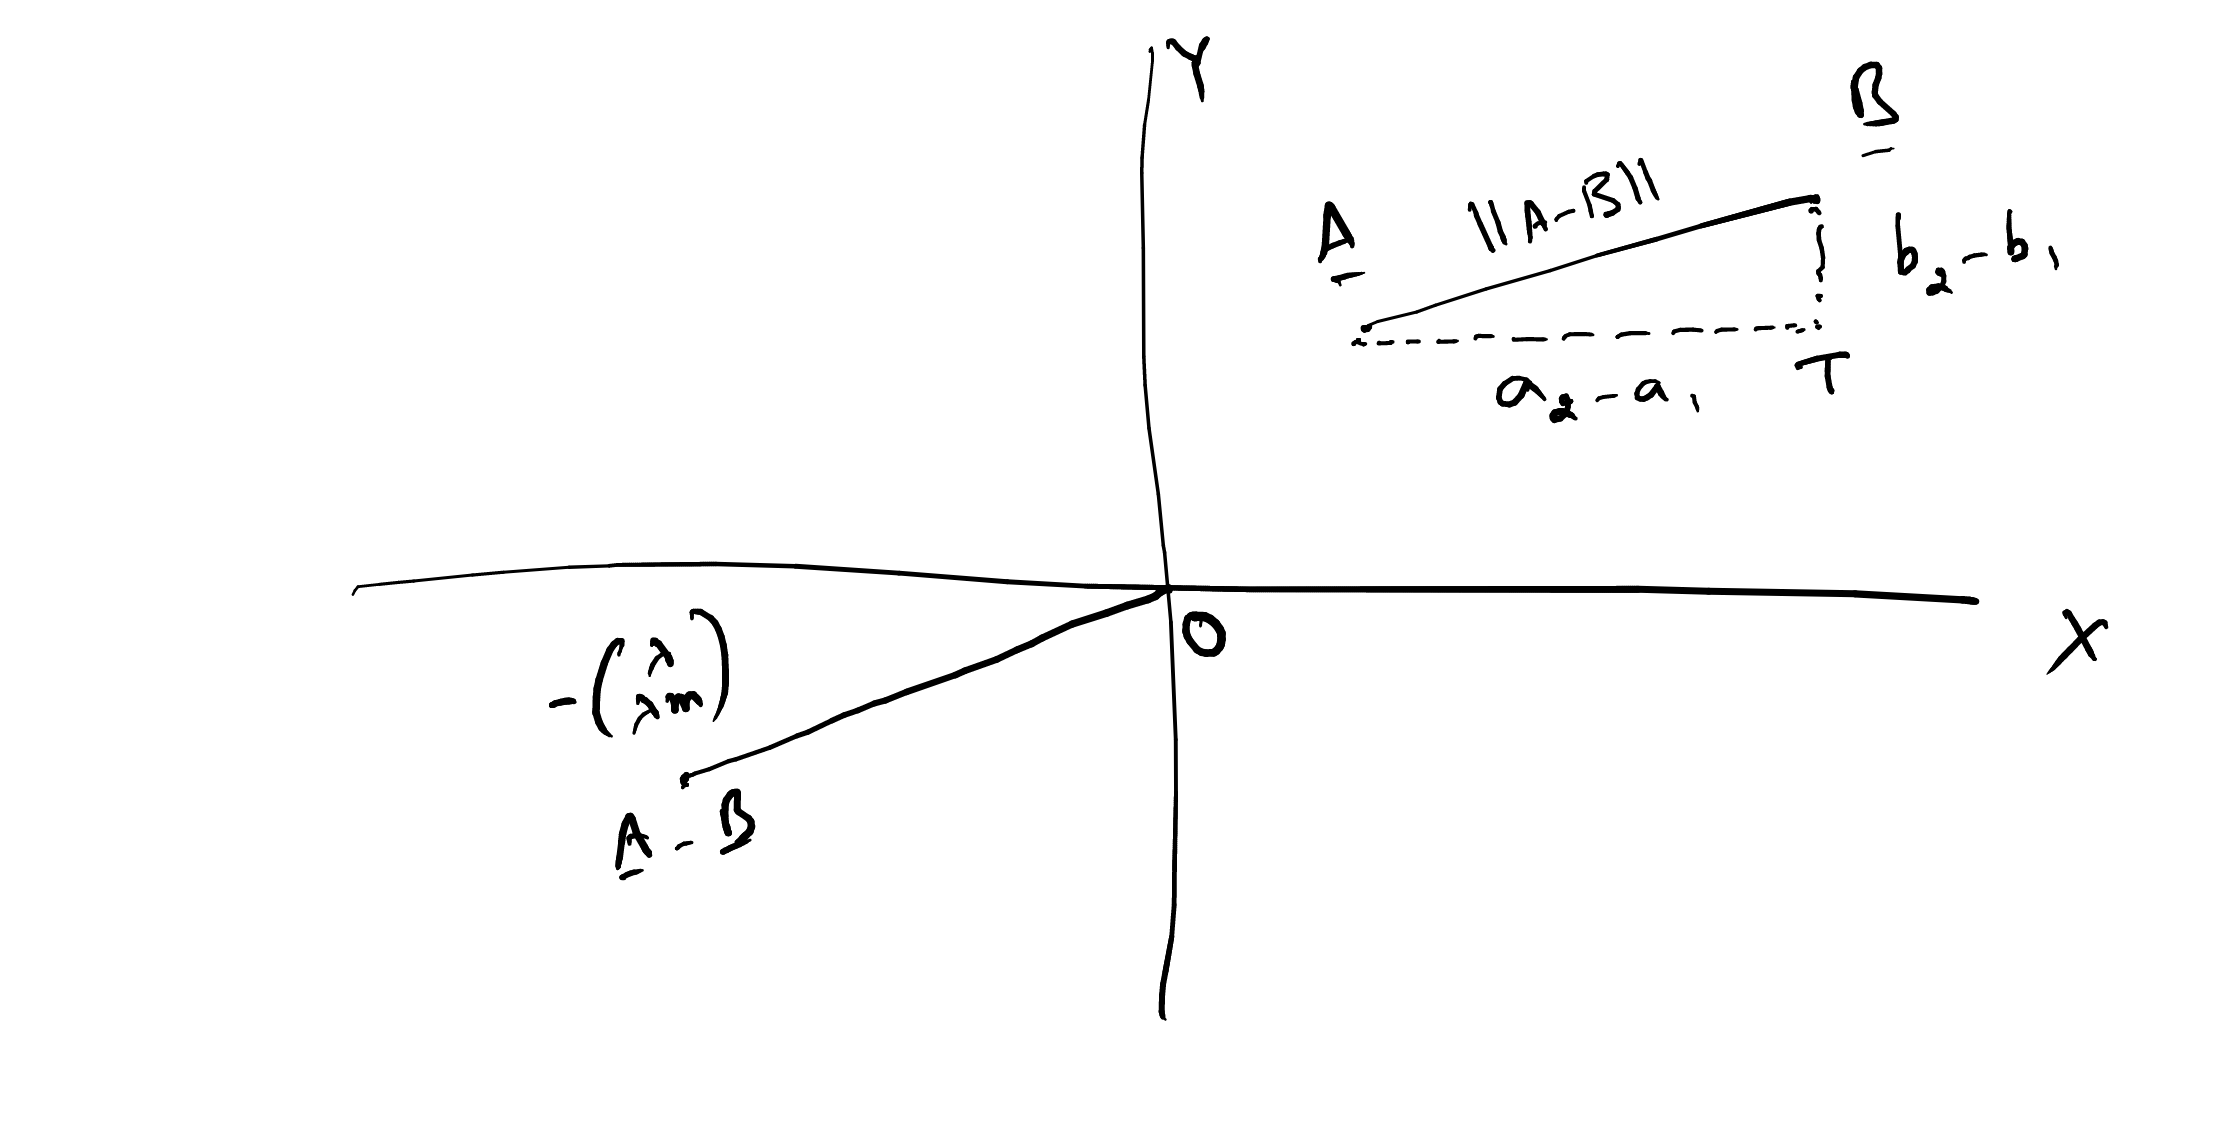
\includegraphics[width=\columnwidth]{./figs/ab.eps}
\caption{}
\label{fig:ab}
\end{figure}
%
\\
\solution See Fig. \ref{fig:ab}. From \eqref{eq:nhomog}, for some 
$\lambda$,
\begin{align}
\vec{B} &=\vec{A} + \lambda \myvec{1 \\ m}
\\
\implies \vec{A} - \vec{B} &= - \lambda \myvec{1 \\ m},
\end{align}
%
$\vec{A} - \vec{B}$ is marked in Fig. \ref{fig:ab}.
%
\item Show that $AB = \norm{\vec{A}-\vec{B}}$
\item Show that the equation of $AB$ is
\begin{align}
\label{eq:line_ab}
\vec{x} = \vec{A}+ \lambda\brak{\vec{B}-\vec{A}}
\end{align}
%
\item The {\em normal} to the vector $\vec{m}$ is defined as
\begin{align}
\label{eq:normal}
\vec{n}^T\vec{m} = 0
\end{align}
\begin{align}
\label{eq:normal_omat}
\vec{n} = \myvec{0 & 1\\ -1 & 0}\vec{m}
\end{align}
\item From \eqref{eq:line_ab}, the equation of a line can also be expressed as
\begin{align}
\label{eq:line_ab_normal}
\vec{n}^T\vec{x} &= \vec{n}^T\vec{A}+ \lambda\vec{n}^T\brak{\vec{B}-\vec{A}}
\\
\implies \vec{n}^T\vec{x} &=c
\end{align}
\item The unit vectors on the $x$ and $y$ axis are defined as
\begin{align}
\label{eq:line_unit}
\vec{e}_1 &=\myvec{1\\0}, 
\\
\vec{e}_2 &=\myvec{0\\1}
\end{align}
\item If $a$ be the {\em intercept} of the line 
\begin{align}
\label{eq:line_intercept}
\vec{n}^T\vec{x} &=c
\end{align}
on the $x-$axis, then $\myvec{a\\0}$  is a point on the line.  Thus, 
\begin{align}
\label{eq:line_intercept}
\vec{n}^T\myvec{a\\0} &=c
\\
\implies a &= \frac{c}{\vec{n}^T\vec{e}_1}
\end{align}
%
\renewcommand{\theequation}{\theenumi}
%
\item The {\em rotation matrix} is defined as
\begin{align}
\vec{Q} = \myvec{\cos \theta & -\sin \theta\\ \sin \theta & \cos \theta}
\end{align}
%
where $\theta$ is anti-clockwise.
\item 
\begin{align}
\vec{Q}^T\vec{Q} = \myvec{1 & 0 \\ 0 & 1} = \vec{I}
\end{align}
%
where $\vec{I}$ is the {\em identity matrix}. The rotation matrix $\vec{Q}$ is also an {\em orthogonal matrix}.

\numberwithin{equation}{enumi}
%
\item Find the equation of  line $L$ in Fig. \ref{fig:line_dist}.
\\
\solution The equation of the $x-$axis is
\begin{align}
\vec{x} =\lambda \vec{e}_1
\end{align}
Translation by $p$ units along the $y-$axis results in 
\begin{align}
L_0: \quad \vec{x} = \lambda \vec{e}_1 + p \vec{e}_2 
\end{align}
Rotation by $90\degree-\alpha$ in the anti-clockwise direction yields
\begin{align}
L: \quad \vec{x} &= \vec{Q}\cbrak{\lambda \vec{e}_1 + p \vec{e}_2 }
\\
&=\lambda \vec{Q}\vec{e}_1 + p \vec{Q}\vec{e}_2 
\label{eq:line_dist_temp}
\end{align}
%
where 
\begin{align}
\vec{Q} &= \myvec{\cos \brak{\alpha-90} & -\sin \brak{\alpha-90}\\ \sin \brak{\alpha-90} & \cos \brak{\alpha-90}}
\\
&= \myvec{\sin \alpha & \cos \alpha \\ -\cos \alpha & \sin \alpha}
\end{align}
%
From \eqref{eq:line_dist_temp},
\begin{align}
L: \quad \vec{e}_2^T\vec{Q}^T\vec{x}&=\lambda \vec{e}_2^T\vec{Q}^T\vec{Q}\vec{e}_1 + p \vec{e}_2^T\vec{Q}^T\vec{Q}\vec{e}_2 
\nonumber \\
&=\lambda \vec{e}_2^T\vec{e}_1 + p \vec{e}_2^T\vec{e}_2 
\end{align}
resulting in 
\begin{align}
L: \quad \myvec{\cos \alpha & \sin \alpha}\vec{x}=p
\label{eq:line_dist_temp_final}
\end{align}
\begin{figure}
\centering
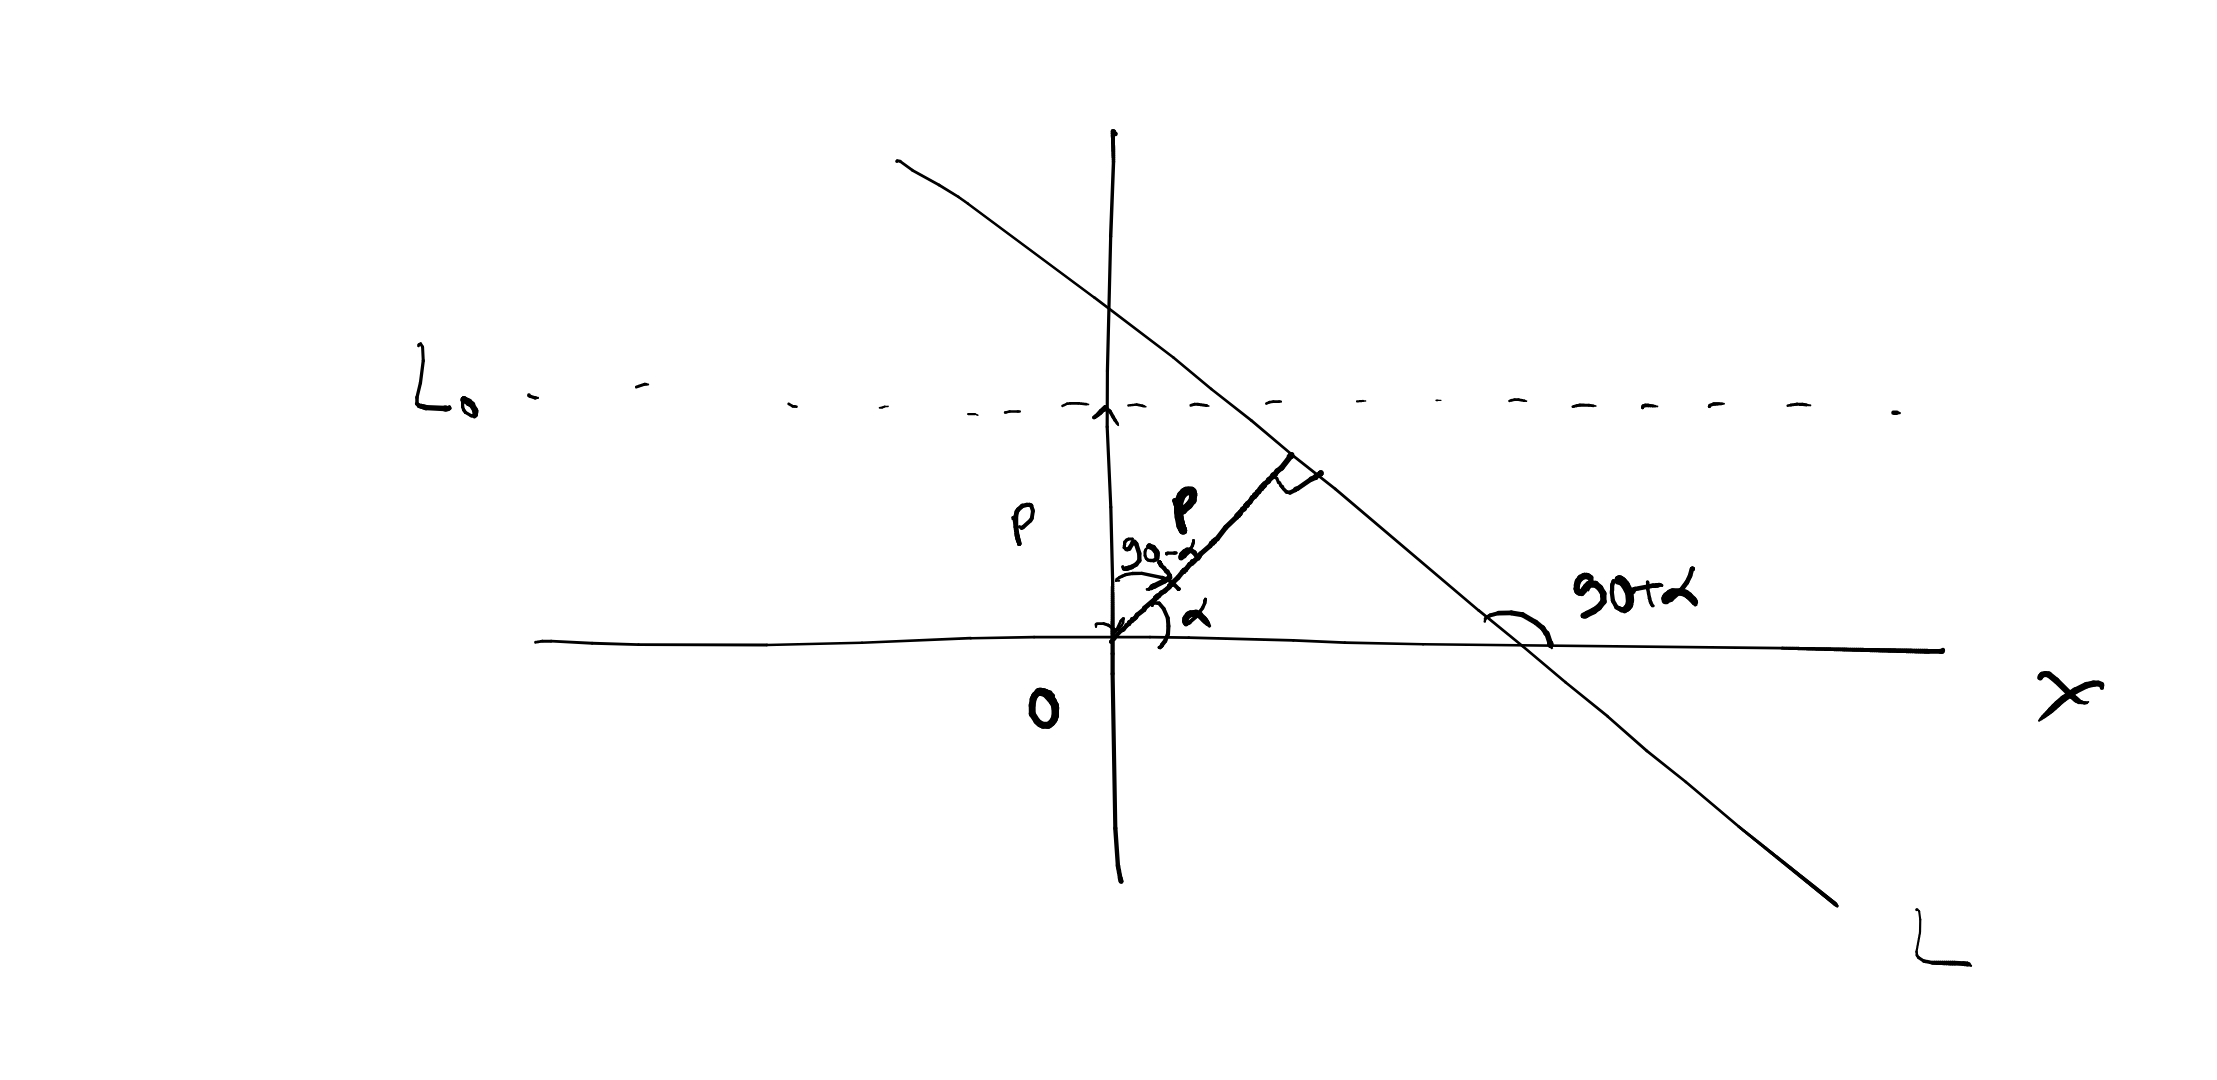
\includegraphics[width=\columnwidth]{./figs/line_dist.eps}
\caption{}
\label{fig:line_dist}
\end{figure}
\item Show that the distance from the orgin to the line 
\begin{align}
\vec{n}^T\vec{x} &=c
\end{align}
is 
\begin{align}
p = \frac{c}{\norm{n}}
\label{eq:line_dist_orig}
\end{align}
\end{enumerate}
%
%\section{Orthogonality}
%\begin{enumerate}[label=\thesection.\arabic*
%,ref=\thesection.\theenumi]
%\item See Fig. \ref{fig:orth}.  In $\triangle ABC, AB \perp BC$. Show that
%\begin{equation}
%\brak{\vec{A}-\vec{B}}^T\brak{\vec{B}-\vec{C}} = 0
%\label{eq:orth}
%\end{equation}
%\begin{figure}
%\centering
%\includegraphics[width=\columnwidth]{./figs/orth.eps}
%\caption{}
%\label{fig:orth}
%\end{figure}
%%
%\solution Using Baudhayana's theorem,
%\begin{align}
%\norm{\vec{A}-\vec{B}}^2 + \norm{\vec{B}-\vec{C}}^2 &= 
%\norm{\vec{C}-\vec{A}}^2
%\\
%\implies 
%\brak{\vec{A}-\vec{B}}^T\brak{\vec{A}-\vec{B}} 
%&+ 
%\brak{\vec{B}-\vec{C}}^T\brak{\vec{B}-\vec{C}} 
%\nonumber \\
%&= 
%\brak{\vec{C}-\vec{A}}^T \brak{\vec{C}-\vec{A}}
%\nonumber \\
%\implies 
%2\vec{A}^T\vec{B} - 2\vec{B}^T\vec{B}&+2\vec{B}^T\vec{C}-2\vec{A}^T\vec{C}
%=0
%\end{align}
%which can be simplified to obtain \eqref{eq:orth}.
%%
%\item Let $\vec{x}$ be any point on $AB$ in Fi.g \ref{fig:orth}.  Show that
%\begin{equation}
%\brak{\vec{x}-\vec{A}}^T\brak{\vec{B}-\vec{C}} = 0
%\end{equation}
%%
%\item If $\vec{x,y}$ are any two points on $AB$, show that 
%\begin{equation}
%\label{eq:orth_any}
%\brak{\vec{x}-\vec{y}}^T\brak{\vec{B}-\vec{C}} = 0
%\end{equation}
%%
%\item In Fig. \ref{fig:alt}, $BE \perp AC, CF \perp AB$.  Show that $AD \perp BC$.
%\begin{figure}[!hb]
%\centering
%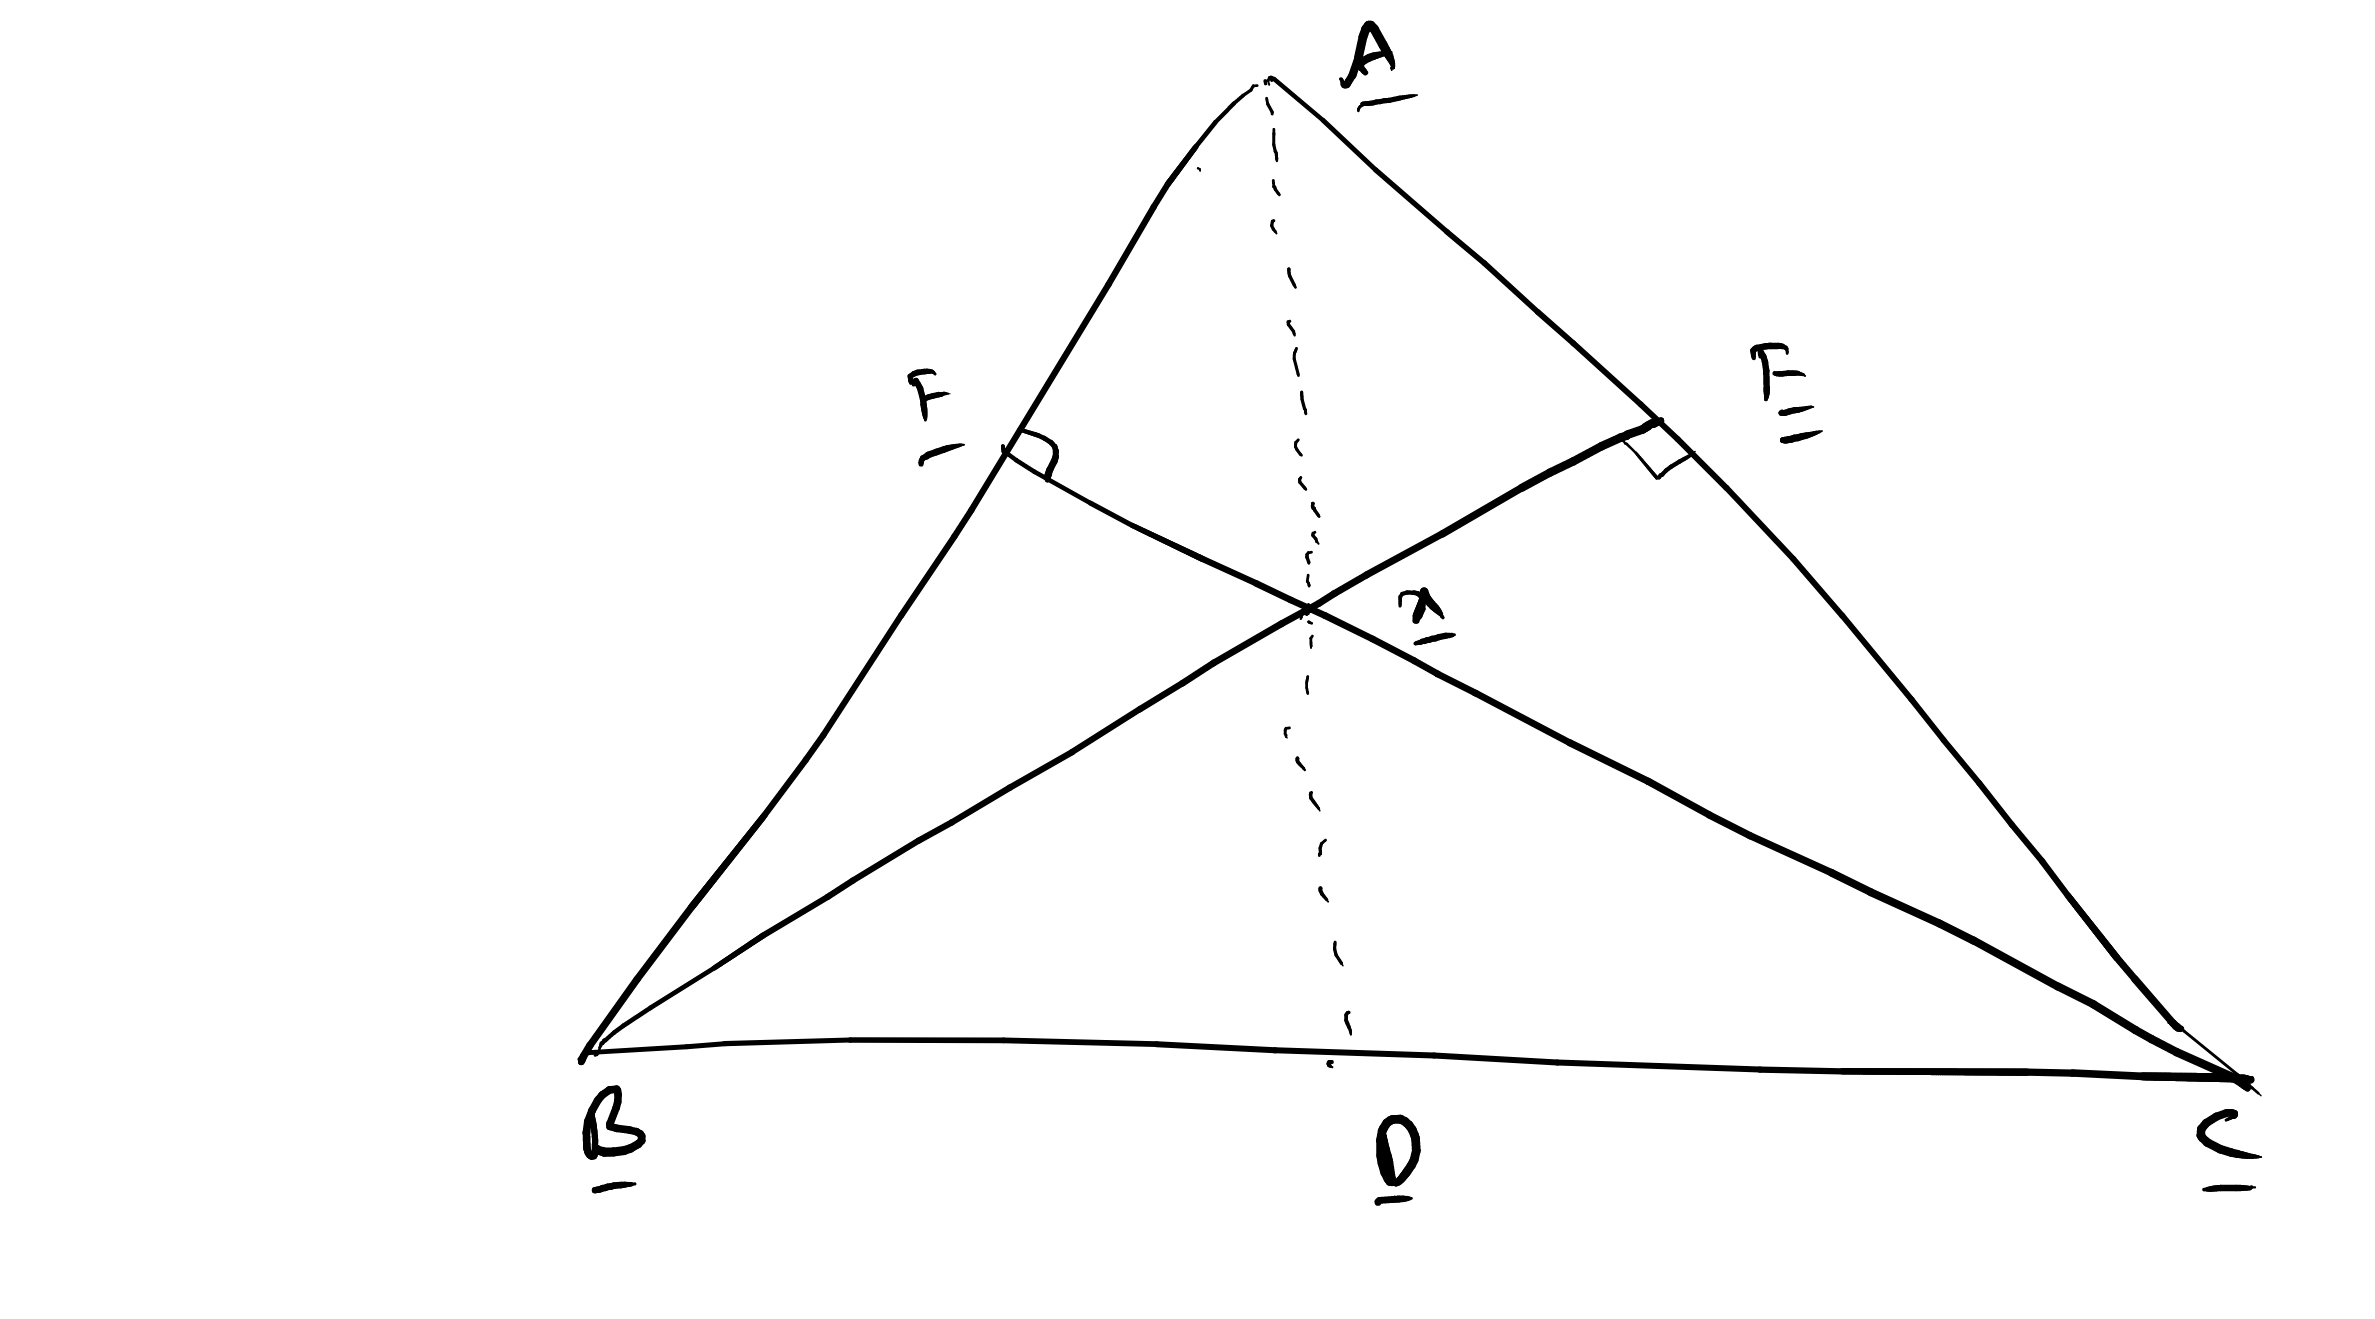
\includegraphics[width=\columnwidth]{./figs/alt.eps}
%\caption{}
%\label{fig:alt}
%\end{figure}
%\\
%\solution Let $\vec{x}$ be the intersection of $BE$ and $CF$. Then, using 
%\eqref{eq:orth_any},
%\begin{align}
%\label{eq:alt_1}
%\begin{split}
%\brak{\vec{x}-\vec{B}}^T
%\brak{\vec{A}-\vec{C}} &= 0
%\\
%\brak{\vec{x}-\vec{C}}^T
%\brak{\vec{A}-\vec{B}} &=0
%\end{split}
%\\
%\label{eq:alt_3}
%\implies \vec{x}^T\brak{\vec{A}-\vec{C}}-\vec{B}^T\brak{\vec{A}-\vec{C}} &= 0
%\\
%\text{and }\vec{x}^T\brak{\vec{A}-\vec{B}}-\vec{C}^T\brak{\vec{A}-\vec{B}} &= 0
%\label{eq:alt_4}
%\end{align}
%%
%Subtracting \eqref{eq:alt_4} from \eqref{eq:alt_3},
%\begin{align}
%\vec{x}^T\brak{\vec{B}-\vec{C}} + \vec{A}^T\brak{\vec{C}-\vec{B}} &= 0
%\\
%\implies \brak{\vec{x}^T - \vec{A}^T}\brak{\vec{B}-\vec{C}}  &= 0
%\\
%\implies \brak{\vec{x} - \vec{A}}^T\brak{\vec{B}-\vec{C}}  &= 0
%\end{align}
%%
%which completes the proof.
%\end{enumerate}
%
%\section{Medians of a triangle}
%\begin{enumerate}[label=\thesection.\arabic*
%,ref=\thesection.\theenumi]
%\item In Fig. \ref{fig:ratio},
%\begin{equation}
%\frac{AB}{BC} = \frac{\norm{\vec{A}-\vec{B}}}{\norm{\vec{B}-\vec{C}}} = k.
%\label{eq:k}
%\end{equation}
%%
%Show that
%%
%\begin{equation}
%\frac{\vec{A}+k\vec{C}}{k+1} = \vec{B}.
%\label{eq:ratio}
%\end{equation}
%%
%\begin{figure}[!hb]
%\centering
%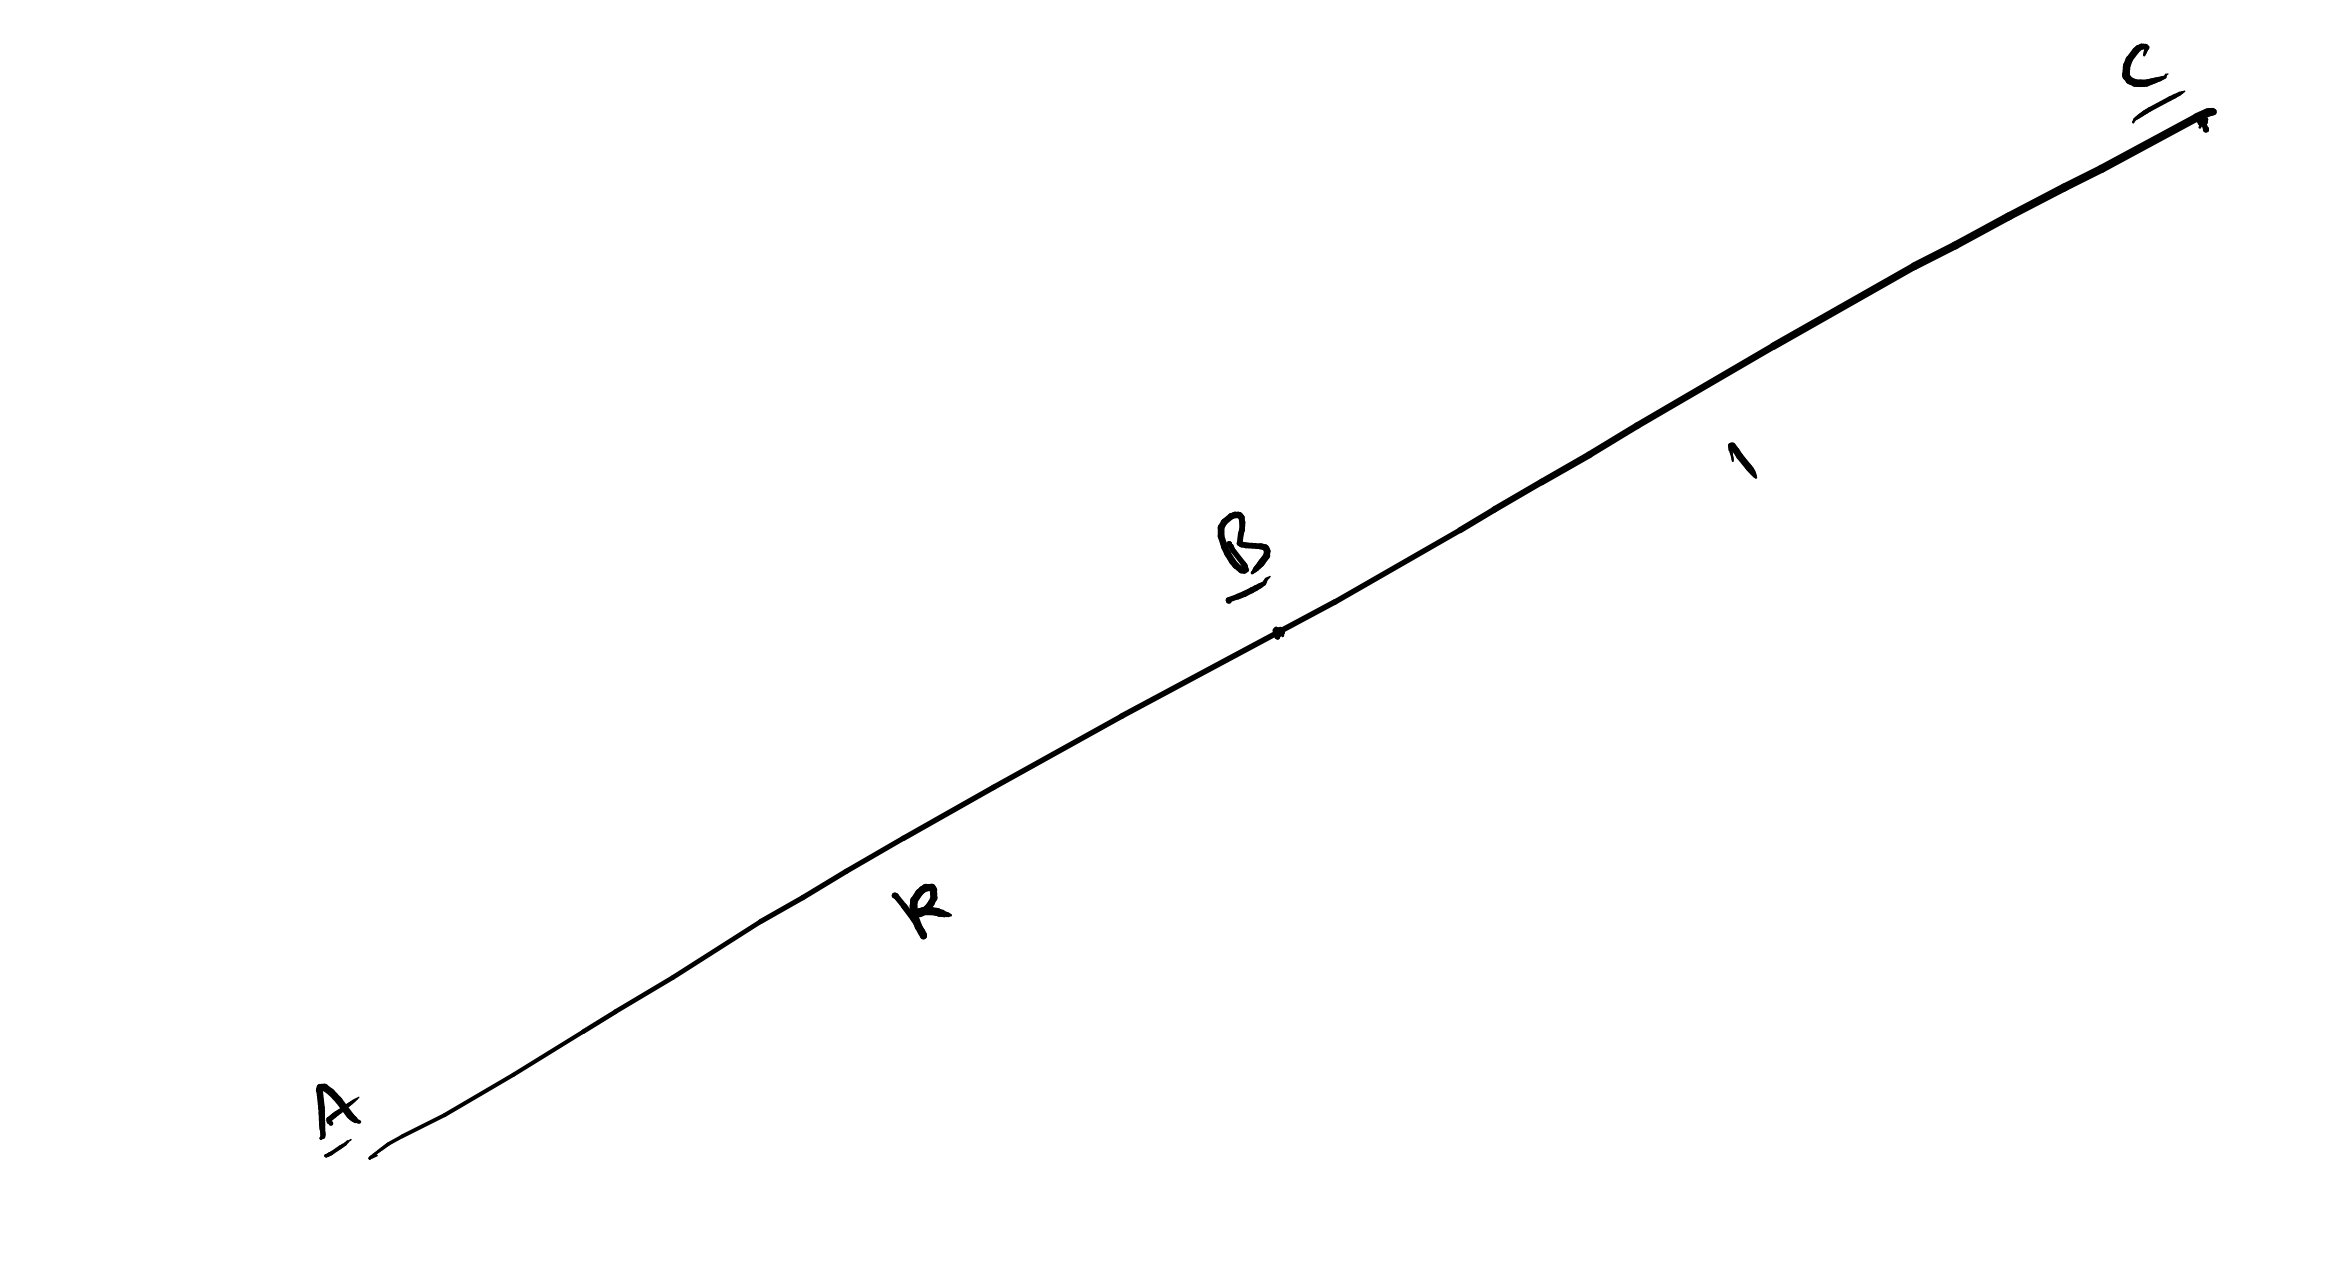
\includegraphics[width=\columnwidth]{./figs/ratio.eps}
%\caption{}
%\label{fig:ratio}
%\end{figure}
%\solution From \eqref{eq:nhomog}, 
%\begin{align}
%\begin{split}
%\vec{B} &= \vec{A} + \lambda_1 \myvec{1 \\ m},
%\\
%\vec{B} &= \vec{C} - \lambda_2 \myvec{1 \\ m}.
%\end{split}
%\\
%\label{eq:rat_1}
%\implies \frac{\norm{\vec{A}-\vec{B}}}{\norm{\vec{B}-\vec{C}}} &= 
%\frac{\lambda_1}{\lambda_2} = k
%\\
%\text{and } \frac{\vec{B}- \vec{A}}{\lambda_1} &= \frac{\vec{C}- 
%\vec{B}}{\lambda_2} =  \myvec{1 \\ m},
%\label{eq:rat_2}
%\end{align}
%%
%from \eqref{eq:k}. Using \eqref{eq:rat_1} and \eqref{eq:rat_1},
%\begin{align}
%\vec{A}- \vec{B} &=  k\brak{\vec{B}- \vec{C}}
%\end{align}
%%
%resulting in \eqref{eq:ratio}.
%%
%\item If $\vec{A}$ and $\vec{B}$ are linearly independent,  
%\begin{equation}
%k_1\vec{A} + k_2\vec{B} = 0 \implies k_1=k_2=0
%\end{equation}
%\item $BE$ and $CF$ are medians of $\triangle ABC$ intersecting at $O$ as shown in Fig. \ref{fig:median}. 
%Show that
%\begin{equation}
%\frac{CO}{OF} = \frac{BO}{OE} = 2
%\end{equation}
%%
%\begin{figure}[!hb]
%\centering
%\includegraphics[width=\columnwidth]{./figs/median.eps}
%\caption{}
%\label{fig:median}
%\end{figure}
%\solution Let
%\begin{align}
%\frac{CO}{OF} &= k_1
%\\
%\frac{BO}{OE} &= k_2
%\end{align}
%%
%Using  \eqref{eq:ratio},
%\begin{align}
%\vec{E}&= \frac{\vec{A} + \vec{C}}{2}
%\\
%\vec{F}&= \frac{\vec{A} + \vec{B}}{2}
%\end{align}
%%
%and
%\begin{align}
%\label{eq:o1}
%\vec{O}&= \frac{k_1\vec{F} + \vec{C}}{k_1+1} = \frac{k_1\frac{\vec{A} + \vec{B}}{2} + \vec{C}}{k_1+1}
%\\
%\vec{O}&= \frac{k_2\vec{E} + \vec{B}}{k_2+1} = \frac{k_2\frac{\vec{A} + \vec{C}}{2} + \vec{B}}{k_2+1}
%\label{eq:o2}
%\end{align}
%%
%From \eqref{eq:o1} and \eqref{eq:o2},
%\begin{align}
% \frac{k_1\frac{\vec{A} + \vec{B}}{2} + \vec{C}}{k_1+1} &= 
% \frac{k_2\frac{\vec{A} + \vec{C}}{2} + \vec{B}}{k_2+1}
%\end{align}
%\begin{multline}
%\label{eq:lin_comb}
%\implies \sbrak{\frac{k_1\brak{k_2+1}}{2}
%-\frac{k_2\brak{k_1+1}}{2}}\vec{A} 
%\\
%+ 
%\sbrak{\frac{k_1\brak{k_2+1}}{2}-\brak{k_1+1}}\vec{B} 
%\\
%+ \sbrak{\brak{k_2+1}-\frac{k_2\brak{k_1+1}}{2}}\vec{C} 
%= 0
%\end{multline}
%resulting in $k_1 = k_2$,
%\begin{align}
%k_1^2-k_1-2  &= 0
%\implies k_1 = k_2 = 2,
%\end{align}
%provided $\vec{A},\vec{B},\vec{C}$ are linearly independent. Thus, substituting $k_1=2$ in \eqref{eq:o2},
%\begin{equation}
%\vec{O} = \frac{\vec{A}+\vec{B}+\vec{C}}{3}
%\end{equation}
%%
%If $\vec{A},\vec{B},\vec{C}$ are linearly dependent,
%\begin{align}
%\label{eq:lin_dep}
%\vec{A} = \alpha \vec{B} + \beta \vec{C} 
%\end{align}
%%
%Note that $\vec{B},\vec{C}$ are linearly independent.
%Substituting \eqref{eq:lin_dep} in \eqref{eq:lin_comb},
%\begin{multline}
%%\label{eq:lin_comb}
% \sbrak{\frac{k_1\brak{k_2+1}}{2}
%-\frac{k_2\brak{k_1+1}}{2}}\sbrak{\alpha \vec{B} + \beta \vec{C}  }
%\\
%+ 
%\sbrak{\frac{k_1\brak{k_2+1}}{2}-\brak{k_1+1}}\vec{B} 
%\\
%+ \sbrak{\brak{k_2+1}-\frac{k_2\brak{k_1+1}}{2}}\vec{C} 
%= 0
%\end{multline}
%\begin{align}
%\implies
%\begin{split}
%\brak{k_1-k_2}\alpha + k_1k_2 - k_1-2 &=0
%\\
%\brak{k_1-k_2}\beta - k_1k_2 + k_2+2 &=0
%\end{split}
%\label{eq:median_contra}
%\\
%\implies \brak{k_1-k_2}\brak{\alpha +\beta - 1} = 0
%\end{align}
%If $\alpha+\beta = 1, \vec{A},\vec{B},\vec{C}$ are collinear according to \eqref{eq:ratio} resulting in a 
%contradiction.  Hence, $k_1=k_2$, which, upon substitution in \eqref{eq:median_contra}, yields
%\begin{equation}
%k_1^2 - k_1-2 = 0 \implies k_1 = 2.
%\end{equation}
%\end{enumerate}
